\documentclass{polytech/polytech}
\usepackage{pdfpages}
% zone du préambule
\typereport{ppgldi4}

\reportyear{2017-2018}

\title{Création de fond de planning}
% https://gitlab.projectsforge.org/polytech/polytech/wikis/home

\student{Hanyuan}{Peng}{hanyuan.peng@etu.univ-tours.fr}
\student{Stéphane}{Deluce}{stephane.deluce@etu.univ-tours.fr}

\academicsupervisor[di]{Christophe}{Lenté}{christophe.lente@univ-tours.fr}

\resume{Le programme devra créer un fond de planning en Excel afin de faciliter la création des emplois	du temps. Grossièrement, le fond de de planning se présente comme un quadrillage avec en ligne les cours (CM, TD, TP) et en colonne les semaines. Des formules de calculs sont ajoutées à certaines cases afin de comptabiliser les heures placées. Le programme prendra en entrée un fichier excel (ou au pire csv) contenant une maquette et les enseignants affectés. Il fournira en sortie un fichier excel.}
\motcle{Java}
\motcle{Excel}
\motcle{Apache POI}

\abstract{This is an example of an abstract for the report.}
\keyword{Java}
\keyword{Excel}
\keyword{Apache POI}


% zone du préambule
\begin{document}
	% zone du contenu du document
	\part{Introduction}
	\section{Présentation du projet}
	ici expliquer le projet, son but ...
	
	\part{Environnement de développement}
	Eclipse, java car imposé …
		
	\section{Outils de gestion de projet}
	Git (GitLab), Trello, maven (gestionnaire de dependances)
	
	\part{Étude de projet}
	\section{Analyse des besoins}
	Expliquer les fonctions principales du projets … (formules, mise en formes)
	
	\section{Spécifications Fonctionnelles}
	
	\section{Modélisation}
	Expliquer notre choix de design pattern.
	
	\subsection{UML}
	
	\subsection{Définitions des classes}
	
	\part{Planification}
	
	\section{Découpage en taches}
	
	\section{Répartition des tâches}
	
	Nous avons choisi de se diviser le travail par classes.
	Avec des points régulier pour expliquer l'avancé de notre travail, et partager nos remarques et
	interrogations
	
	\part{Implémentation}
	
	Expliquer notre choix, formules, documentation, ...
	
	\section{Organisation}
	
	\subsection{Organisation des fichiers}
	
	Nous avons commencé par développer les modèles, puis les contrôleurs pour finir avec la vue.
	Tests unitaires ont étés réalisés après l'écriture de chaques méthodes de chaques classes.
	
	\section{Tests et validation}
	
	\section{Documentation}
	
	Classes documentés pour évolutivité, ...
	
	\part{Annexes}
	
	\section{Manuel d'utilisation}
	\includepdf[pages=3-, offset=0 0]{../manuel.pdf}
\end{document}